\setchapterpreamble[u]{\margintoc}
\chapter{The Falling Raindrop}
\labch{raindrop}

The focus of the present chapter shall be to take a closer look at the issues 
plaguing numerical methods that try to deal with flows 
entailing significant density contrasts between the fluids. 
Arguably, the most common instances of such flows are those involving the interaction
between air and water, primarily in the form of droplets and 
bubbles that play important roles in both natural and industrial processes. 
As for the numerical platform, we use `PARIS Simulator' 
\sidenote{Refer to \cite{paris} for a detailed exposition  
of the numerical methods implemented in `PARIS Simulator.} 
to carry out our simulations on this topic. 
A flow configuration that combines the complexities of large 
density-ratios with the interaction between capillary, viscous and 
inertial stresses is that of a water droplet falling in 
air under the influence of gravitational acceleration.

%---------------------------------------------------------------
\section{Problem Setup}

The problem is characterized by a combination of Reynolds, 
Weber and Bond numbers, the definitions of which are as follows : 

\begin{align}
	\textrm{We}=\frac{\rho_{g} U^2 D}{\sigma} \quad,\quad \textrm{Re}= \frac{\rho_{l} U D}{\mu_{g}} \quad,\quad \textrm{Bo}=\frac{\left(\rho_{l}-\rho_{g}\right) g D^2 }{\sigma}
\end{align}

\marginnote{As the density and viscosity ratios are corresponding to that of air-water systems at 20 degree Celcius,
an equivalent characterization could be done using the Morton number $\left( \textrm{Mo} = \frac{g\mu_g^4(\rho_l-\rho_g)}{\rho_g^2 \sigma^3} \right)$ 
in place of the Bond number.}


The subscripts $l$ and $g$ represent liquid and gas phases respectively. 
In our particular numerical setup, $\textrm{We}\simeq 3.2 $, 
$\textrm{Re} \simeq 1455 $ and $\textrm{Bo} \simeq 1.2 $,
thus corresponding to that of a $3mm$ diameter raindrop (a relatively large one) 
falling in the air at an approximate terminal velocity of  
$8$ m/s (interpolated from empirical data, refer to Gunn and Kinzer \cite{gunn1949}). 
This choice of length scale of the drop is motivated by the paradigmatic value
of a near-spherical raindrop simulation, and by the fact that the corresponding Weber
number ($\sim 3$) is the same as in a similar air-water setup corresponding to  
suddenly-accelerated-droplet (or ``secondary atomization" ) simulations in the studies \cite{xiao2012,xiao2014large}.
For such a low Weber number the capillary forces dominate and the 
droplet should remain intact, and definitely not undergo any subsequent atomization. 
The parameters in the problem setup are given in Table \ref{raindropprop}, 
and the schematic diagram given in Fig. \ref{setup}. 
The droplet is initially placed at the center of a cubic domain (3D), 
where the length of the side is 4 times the diameter of the drop. 

\begin{table*}[h!]
\begin{center}
\begin{tabular}{ccccccc}
\hline\hline
$\rho_{g}$ & $\rho_{l}$ & $\mu_{g}$ 
& $\mu_{l}$ & $\sigma$ & $D$ & $g$\\
$\left(kg/m^3\right)$ & $\left(kg/m^3\right)$ & $\left(Pa \, s\right)$ 
& $\left(Pa \,s \right)$ & $\left(N/m\right)$ & $(m)$ & $(m /s^{2})$ \\
\hline
1.2 & $0.9982 \times 10^3$ & $1.98 \times 10^{-5}$ & 
$8.9 \times 10^{-4}$ & $0.0728$ & $3 \times 10^{-3}$ & $9.81$\\
\hline\hline
\end{tabular}
\caption{Parameter values used in the simulation 
	of a falling water droplet in air. \label{raindropprop}}
\end{center}
\end{table*}


In order to properly reproduce and analyse the dynamics 
of a relatively large drop (high Reynolds flow) such as in our case, 
the numerical method has to accurately resolve the thin boundary layers 
\sidenote{Even for simulations with 60 points across the droplet diameter, 
the boundary layer has only by 3-4 cells across it. }, 
the interaction of such layers with the capillary forces and finally 
the non-linear feedback of the complex 
3D vortical structures present in the wake behind the droplet.
Arguably, the most natural type of computational setup would involve using 
a large domain filled with air at rest, with zero inflow velocity and to
let the droplet fall from the top of the domain.
Such an undertaking was attempted by Dodd and Ferrante \cite{dodd2014}, 
in which they managed to delineate the different regimes concerning the 
behavior of the wake behind the droplet, although at relatively 
lower Reynolds numbers corresponding to smaller drops 
(the maximum Reynolds tested was $\simeq 500$, whereas in our case it is $\simeq 1500$).    
We on the other hand use a significantly smaller domain ($L/D = 4$ where $L$ is the domain size), 
with a constant value of inflow velocity (close to $8$ m/s), thus resulting in the drop 
exiting the domain after a certain amount of time. 
This setup proves to be quite convenient for relatively short-time investigations.
Therefore, our objective behind the demonstration of this particular 
test case is \textit{not} to develop a high fidelity model of a raindrop 
\sidenote{In the Dodd and Ferrante \cite{dodd2014} study , 
a droplet was allowed to fall from rest
along a domain with a length corresponding to 32 times the droplet diameter, 
therefore necessitating a problem size of approximately 260 million cells.}, 
but rather carry out a stringent evaluation of the robustness of our class of 
numerical methods (shifted fractions and sub-grid strategies) 
compared to the standard version of the method that is not mass-momentum consistent. 

% -----
\begin{figure}[h!]
\begin{center}
\includegraphics[width=0.5\textwidth]{plots/raindrop/setup.png}
\end{center}
\caption{A 2D schematic of the numerical setup for the falling raindrop. 
	A droplet of diameter $D$ is placed at the center of a cubic domain 
	of side $L$ and $L/D = 4$. The liquid properties ($\rho_l$ , $\mu_l$) 
	correspond to that of water, and the gas properties ($\rho_g$,$\mu_g$) 
	correspond to that of air. We apply a uniform inflow velocity condition 
	with $U_0(t)$ and an outflow velocity condition at the top which 
	corresponds to zero normal gradient.
	Boundary conditions on the side walls correspond 
	to those of impenetrable free slip (no shear stress).}
\label{setup}
\end{figure}

%---------------------------------------------------------------
\section{Numerical Instabilities}

Numerical simulations using a fixed inflow velocity with $U_0(t) = 8 $ m/s 
were carried out for very short times (of the order of 1ms) at moderate resolution 
\sidenote{Droplet resolutions between $D/h = 16$ to $D/h = 64$ are considered
to be moderate, where $D$ is the droplet diameter and $h$ is the grid size.}.
The simulations carried out with the standard version of our numerical method 
result in the catastrophic deformations of the droplet as illustrated in Fig. \ref{explode_compare}, 
which we describe as ``fictitious" or ``artificial" atomization. 
They display marked peaks or spikes in kinetic energy as a function of time, 
associated with massively deformed interface shapes (see figure \ref{explode_compare}). 
Additionally, our studies suggest that certain combinations 
of the advection scheme and the flux limiter are 
numerically more robust than others
,in particular, the most stable combinations 
are that of CIAM advection with 
Superbee limiter, and the WY advection with QUICK limiter. 

\subsection*{Instability Mechanism}

We propose the following explanation in order to account for such numerical artifacts. 
To start with, we neglect gravity and viscous effects at this relatively large Reynolds number. 
Also, we are interested in steady-state flow 
\sidenote{As the simulation starts with uniform flow in the gas and a zero velocity
in the drop, there is a sudden large acceleration in the gas, resulting in the development 
of a dipolar velocity field akin to that of potential flow around a cylinder (sphere). }. 
On the axis and near the hyperbolic stagnation point 
at the front of the droplet one has $u_2=0$ for the transverse 
(radial) velocity and for the axial momentum balance


\begin{align}
u_1 \partial_1 u_1 = - \frac 1 \rho \partial_1 p.
\end{align}

Due to the large viscosity and density ratios, it is not possible for 
the air flow to immediately entrain the water, so the fluid velocity 
is significantly smaller inside the droplet. 
In the air the acceleration near the stagnation point is 
of the order $U^2/D$, whereas the pressure gradient is

\begin{align}
\partial_1 p \sim \rho_{g} U^2/D.
\end{align}

The pressure gradient in the liquid is much smaller, 
however, in the case of a mixed cell the water density 
may multiply (due to numerical errors) with the gas acceleration $U^2/D$, so that

\begin{align}
\partial_1 p \sim \rho_{l} U^2/D,
\end{align}

then a large pressure gradient results in the mixed cell or cells. 
This large pressure gradient results in pressure spikes inside the 
droplet near the front stagnation point, as shown in Figure \ref{pressure_1}. 
Such pressure gradients are balanced by surface tension only for a sufficiently 
large curvatures near the droplet front. 
This explains the presence of a ``dimple'' often observed in low 
resolution simulations of the falling drop. 
This artifact had been observed by Xiao \cite{xiao2012} in a similar case
\sidenote{In the thesis of Xiao, the focus was on the analysis of droplet breakup 
corresponding to different Weber number regimes.}
involving the sudden interaction of a droplet at rest with a uniform gas flow. 
The resulting large un-physical pressure gradients across the interface 
eventually lead to its rapid destabilization and concomitant breakup.  

\begin{figure*}
\begin{center}
\begin{tabular}{cc}
\hspace*{-1.0cm}
\includegraphics[width=0.8\textwidth]{plots/raindrop/pressure_compare.png} &
\hspace{-0.4cm}%
\includegraphics[width=0.8\textwidth]{plots/raindrop/nonmc_16ppd_pressure.png}\\
\hspace{-0.8cm}%
(a) & (b)
\end{tabular}
\end{center}
\caption{The origin of the pressure peak in the front of the droplet. 
(a) The profile of the pressure on the axis a few timesteps after initialisation 
with the standard, non-consistent method (red curve) and the consistent method based
on the shifted fractions (\textbf{MSHIFT}) strategy (green curve). 
Much larger pressure gradients are present across the interface using the non-consistent method. 
(b) The pressure distribution immediately after the start of the simulation 
using the standard, non-consistent method. The pressure peak has not yet resulted
in the formation of a dimple. In all figures the droplet resolution corresponds to $D/h = 16$.
The simulations are carried out with the CIAM advection method, in conjunction with the Superbee limiter.}
\label{pressure_1}
\end{figure*}

\begin{figure*}
\begin{center}
\begin{tabular}{cc}
\hspace*{-1.0cm}
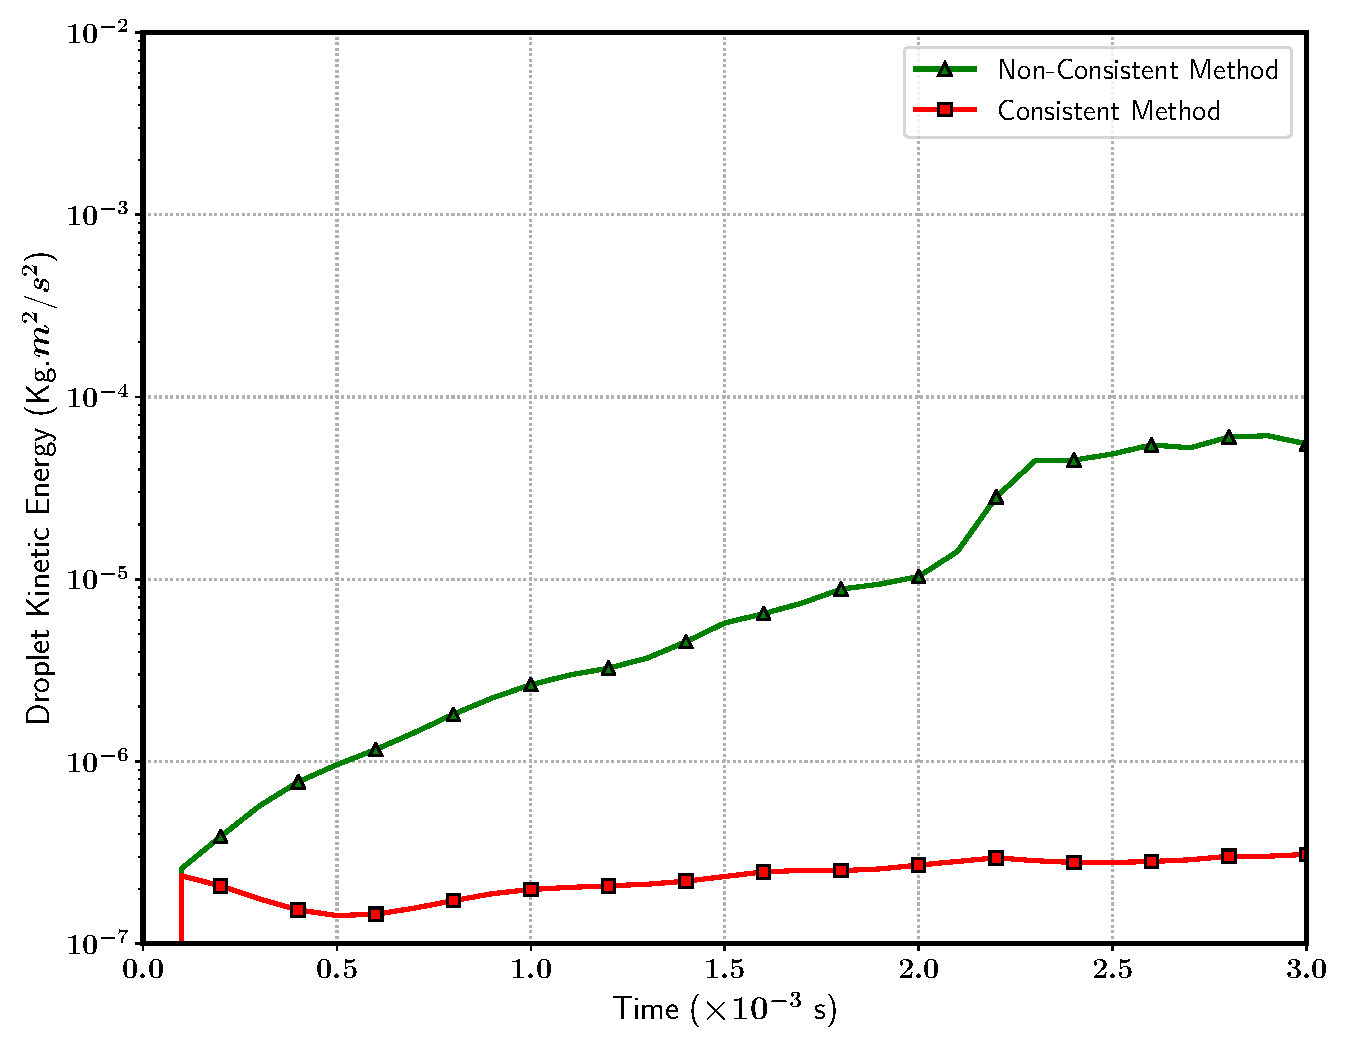
\includegraphics[width=0.8\textwidth]{plots/raindrop/ke_compare.png} &
\hspace{-0.4cm}%
\includegraphics[width=0.8\textwidth]{plots/raindrop/mc_16ppd_pressure.png}\\
\hspace{-0.8cm}%
(a) & (b)
\end{tabular}
\end{center}
\caption{ (a) Comparison of the temporal evolution of droplet kinetic energy. 
The standard non-consistent method displays spikes in the kinetic energy that are 
approximately 3 orders of magnitude larger than that of the consistent method, 
leading to rapid destabilization. 
(b) The pressure distribution immediately after the start of the simulation 
using the consistent method based on the shifted fractions (\textbf{MSHIFT}) strategy. 
In all figures the droplet resolution corresponds to $D/h = 16$.
The simulations are carried out with the CIAM advection method, in conjunction with the Superbee limiter.}
\label{pressure_2}
\end{figure*}

\begin{figure*}
\begin{center}
\begin{tabular}{cc}
\hspace*{-1.0cm}
\includegraphics[width=0.8\textwidth]{plots/raindrop/mc_vorticity_zoom.png} & 
\hspace{-0.4cm}%
\includegraphics[width=0.8\textwidth]{plots/raindrop/mc_vorticity.png} \\ 
\hspace{-0.8cm}%
(a) & (b)
\end{tabular}
\end{center}
\caption{Flow field around the $3 mm$ droplet with $D/h = 16$ immediately 
after the start of the simulation with the consistent method (\textbf{MSHIFT}), 
demonstrating the contours of the norm of the vorticity field (black lines) . 
The 2D cross-section in these figures corresponds to the 
mid-plane slice along the Z axis, where the inflow is along 
the X axis and gravity opposite to it. (a) The velocity magnitude. 
As one can observe, the boundary layer is resolved by only 2-3 cells. 
(b) The velocity component in the Y direction, perpendicular to the flow. 
As the flow develops further, a marked separation of the boundary layers is observed with 
a more complex vortical region in the wake.
The figures correspond to simulations carried out with the 
CIAM advection method, in conjunction with the Superbee limiter.}
\label{flow_field}
\end{figure*}


Visualization of the flow around the droplets (Figure \ref{flow_field}) 
illustrates the challenging nature of the flow configuration, 
even for such a seemingly simple physical problem. 
As one can observe, the thin boundary layers are poorly resolved. 
Therefore, even though the velocity field is continuous across the 
interface (in the discrete sense) in the absence of mass transfer, 
there is the appearance of strong velocity variations at the 
scale of the grid size for such coarse levels of grid refinement. 

\begin{figure*}
\begin{center}
\includegraphics[width=1.25\textwidth]{plots/raindrop/raindrop_explode.png}
\end{center}
\caption{A comparison of the temporal evolution between the standard 
non-consistent method (top row) and the consistent method based on the 
shifted fractions (\textbf{MSHIFT}) strategy (bottom row), 
using the combination of CIAM advection scheme coupled with the Superbee flux limiter. 
The flow is along the positive X direction, with gravity along the opposite direction. 
The red contour indicates the isosurface of the volume fraction 
field corresponding to a value of $0.5$, whereas the black contours 
surrounding the drop represent isosurfaces of the magnitude of vorticity. 
The raindrop with the non-consistent method displays massive deformations 
leading to artificial breakup as a result of rapidly growing numerical instabilities. 
The droplet resolution for both methods is $D/h = 16$ .
The temporal evolution in case of the sub-grid based consistent method (\textbf{MSUB}) produces 
almost indistinguishable figures (bottom row), hence are not shown here.}
\label{explode_compare}
\end{figure*}


%---------------------------------------------------------------

\section{Stabilization Strategies}

The cascading nature of the numerical instabilities that lead to 
the eventual (un-physical) fragmentation of a droplet is not just a 
cause of concern in the context of modeling a raindrop, but it has important
implications within the more broader scope of 
atomization and other complex fragmentation phenomena. 
Arguably, the most important objective of numerical investigations of physical
phenomena involving fragmentation is the quantification of the size of 
the features that result from a series of topological changes 
A typical example is the statistical distributions of drop sizes. 
As demonstrated in the present study, using the standard non-consistent method  
one observes artificially atomized drops thus leading to the generation of a large number of 
smaller fragments, which if counted, will skew the resulting droplet size 
distributions towards the smaller sizes.
Therefore, we assert that the falling raindrop case serves as a faithful representation of the 
numerous under-resolved features that are typically omnipresent in
numerical studies of complex fragmentation phenomena.  
The inability to discern between the drops resulting from physically consistent 
mechanisms and those that result from numerical fragmentation is exactly
why there is a need to develop numerical schemes that circumvent the occurrence
of such instabilities, especially as there will always be some constraints in computational power.  


\subsection*{Consistent Mass-Momentum Transport}

The most common and brute force approach that one can apply 
in order to suppress or circumvent such numerical instabilities is 
by using a combination of extremely refined meshes coupled with large domains \cite{dodd2014}.
A more computationally efficient approach might be to use a 
conservative formulation
\sidenote{A prerequisite of methods that use consistent mass-momentum transport 
is the formulation of the convective operators in the conservative manner i.e
divergence of fluxes instead of gradients of the primary (discontinuous) variables.} 
of the Navier-Stokes equations, in order
to achieve consistency in the discrete transport of mass and momentum. 
A thorough and detailed exposition of the principles
behind the consistent methods and the different strategies towards achieving consistent
transport has already been covered in the chapter 2.  
We observe that the use of our class of consistent methods 
enables us to stabilize a majority of the numerical
instabilities and bring a systematic improvement over wide range of 
flux limiters (WENO, ENO, Superbee, QUICK, Verstappen) 
and CFL numbers, as evidenced by comparing the figures \ref{pressure_1} and \ref{pressure_2}. 

\begin{figure}
\begin{center}
\includegraphics[width = 1.0\textwidth]{plots/raindrop/combined_failures_raindrop.png}
\end{center}
\vspace*{-0.5cm}
\caption{A juxtaposition of the different manifestations of  
`artificial' atomization one encounters while using the standard 
method (\textbf{STD}) that does not involve consistency between the discrete transport of mass and momentum. 
The red contours indicate the isosurface of the volume fraction 
field corresponding to a value of $0.5$, acting as a good proxy for the exact interfacial position. 
One can clearly observe that the un-physical fragmentation of the raindrop is symptomatic 
of the non-consistent method, systematically across all combinations of flux limiters and advection schemes. 
The symbol ``WY'' in the legend corresponds to those run using 
the Weymouth-Yue advection scheme, and ``CIAM'' corresponds to the CIAM scheme. 
Brief descriptions of these advection schemes can be found in chapter 2.
The implementation of the non-linear flux limiters i.e WENO, ENO, QUICK, Superbee, Verstappen 
correspond to that of well established methods developed to 
deal with hyperbolic conservation laws, for more details refer to the
studies of Leveque \cite{flim_1} and Sweby \cite{flim_2}.
The time stamps are indicative of the moments at which the interface
is the most deformed, and do not necessarily correspond to the moment
at which the code crashes.} 
\label{explode_all}
\end{figure}

% multiplot caf_paper
\begin{figure*}
\begin{center}
\includegraphics[width = 1.5\textwidth]{plots/raindrop/multiplot_raindrop.png}
\end{center}
\vspace*{-0.5cm}
\caption{Temporal evolution of quantities of interest to evaluate the 
	performance of our consistent scheme based on the 
	shifted fractions (\textbf{MSHIFT}) method, for different spatial resolutions. 
	(a) Kinetic energy relative to the droplet center-of-mass as defined in \eqref{drop_ke}. 
	(b) Moment of inertia of the droplet along the flow (X) direction. 
	(c) and (d) Moment of inertia of the droplet along the directions 
	perpendicular to flow (Y,Z), evolution of $I_{yy}$ 
	seems to be more or less identical to $I_{zz}$.}
\label{multi_caf}
\end{figure*}

% multiplot jcp_paper
\begin{figure*}
\begin{center}
\includegraphics[width = 1.5\textwidth]{plots/raindrop/jcp_1.png}
\end{center}
\vspace*{-0.5cm}
\caption{Temporal evolution of quantities of interest to evaluate the 
	performance of our consistent scheme based on the 
	sub-grid (\textbf{MSUB}) method, for different spatial resolutions. 
	(a) Kinetic energy relative to the droplet center-of-mass as defined in \eqref{drop_ke}. 
	(b) Moment of inertia of the droplet along the flow (X) direction. 
	(c) and (d) Moment of inertia of the droplet along the directions 
	perpendicular to flow (Y,Z), evolution of $I_{yy}$ 
	seems to be more or less identical to $I_{zz}$.}
\label{multi_jcp}
\end{figure*}

% acc_conv caf_paper
\begin{figure}
\begin{center}
\includegraphics[width = 1.0\textwidth]{plots/raindrop/dropl_velocity_accel_ppd.png}
\end{center}
\vspace*{-0.5cm}
\caption{Comparison of droplet velocity as a function of time, for different droplet resolutions.
	The simulations were carried out with a consistent scheme based on the 
	shifted fractions (\textbf{MSHIFT}) method, using the WY advection scheme with the QUICK limiter. 
	The droplet velocities correspond to that of their respective center of masses. 
	Inset : Convergence of the droplet acceleration as a function of its resolution, 
	computed using the best linear fit over the temporal variation of their respective velocities. 
	The error bars signify the asymptotic standard error (least-squares) corresponding to the linear fits.} 
\label{drop_vel_caf}
\end{figure}

% acc_conv jcp_paper
\begin{figure}
\begin{center}
\includegraphics[width = 1.0\textwidth]{plots/raindrop/jcp_2.png}
\end{center}
\vspace*{-0.5cm}
\caption{Comparison of droplet velocity as a function of time, for different droplet resolutions.
	The simulations were carried out with a consistent scheme based on the 
	sub-grid (\textbf{MSUB}) method, using the WY advection scheme with the QUICK limiter. 
	The droplet velocities correspond to that of their respective center of masses. 
	Inset : Convergence of the droplet acceleration as a function of its resolution, 
	computed using the best linear fit over the temporal variation of their respective velocities. 
	The error bars signify the asymptotic standard error (least-squares) corresponding to the linear fits.} 
\label{drop_vel_jcp}
\end{figure}


\subsection*{Convergence Study}

For the next set of simulations, we use a fixed inflow velocity setup but with smaller initial velocity.
We systematically vary the resolution from  $D/h = 8, 16, 32 $ and $64$. 
Despite using our consistent methods, simulations at  $D/h = 8$ are sometimes unstable, 
so we use a workaround and use a lower fixed inflow velocity of $U_0=5$ m/s, 
which differs from the expected long term terminal velocity
$U_{t} \simeq $8 m/s used in the previous set of simulations. 
But, it does offer a milder initial condition and allows us to observe the first phase of the (physical)
acceleration towards the final statistical steady state. 
The simulations are carried out for 5 ms (for reasons of computational cost and also in order 
to avoid the droplet getting too close to the domain boundaries) 
and the convergence properties of the numerical system are examined within this time frame. 
A brief review of the relevant time scales are as follows : 

\begin{itemize}
\item The time scale $t_a=D/U_0$ of the air flow around the droplet, around 0.6 milliseconds, much shorter
than the simulation time. 
\item The time $t_w = L/[2(U_t - U_0)] = 3$ms that the droplet would take to travel by half the domain
  the domain once it had reached the terminal velocity. This time is not relevant here since one needs to wait first for the next two times
  before terminal velocity is reached. 
\item The time scale $t_c \simeq 15.1$ms \cite{rayleigh1879a} of capillary oscillations of the droplet shape.
\item The time scale $t_i$ of relaxation to terminal velocity. Using the dynamics \eqref{borda} below, 
	this time is $(\rho_l/\rho_g)\cdot( D/U_t) = 215 ms$, which is much longer than the simulation time. 
\item The time scale $t_\mu$ needed to entrain the internal vortical motion of the liquid under the action of the gas. An estimate this time is  $D^2/\nu_l =  \textrm{Re} D/U_t = 400 ms$.
\end{itemize}

The time of relaxation may be estimated using a simple square-velocity drag law for the droplet. 
We model the droplet motion as a one-dimensional dynamics under the effect of gravity and drag as

\begin{align}
	\rho_l \frac{\pi D^3}6 \frac{\textrm{d}U}{\textrm{d}t} =  \rho_l \frac{\pi D^3}6 g - C_D \rho_g \frac{\pi D^2} 8  U^2, \label{borda}
\end{align}

hence

\begin{align}
\frac{\textrm{d}U}{\textrm{d}t}  = -  \frac 34 \frac {r}{D} (U^2 - U_t^2) = -\frac{U-U_t}{t_i}, \label{dtu}
\end{align}

where for $U \simeq U_t$, thus giving us 

\begin{align}
t_i =  \frac 23 \frac {D}{r U_t}.
\end{align}

% mass conservation caf_paper
\begin{figure*}[h!]
\begin{center}
\begin{tabular}{cc}
\hspace*{-1.0cm}
\includegraphics[width=0.7\textwidth]{plots/raindrop/raindrop_mass_conv_16ppd.png} & 
\hspace{-0.2cm}%
\includegraphics[width=0.7\textwidth]{plots/raindrop/raindrop_mass_conv_clipping.png} \\ 
\hspace{-0.2cm}%
(a) & (b) \\
\hspace*{-1.0cm}
\includegraphics[width=0.7\textwidth]{plots/raindrop/raindrop_mass_conv_resolution.png} & 
\hspace{-0.2cm}%
\includegraphics[width=0.7\textwidth]{plots/raindrop/new.png} \\ 
\hspace{-0.2cm}%
(c) & (d)
\end{tabular}
\end{center}
\caption{Relative change in the mass of the droplet 
as a function of time in plots (a), (b) and (c). 
The simulations are carried out with a resolution of $D/h = 16$, 
for a total time of $0.1$ milliseconds using the consistent 
scheme based on the shifted fractions (\textbf{MSHIFT}) method. 
The symbol ``WY'' in the legend corresponds to those run using 
the Weymouth-Yue advection scheme in combination with the QUICK limiter, 
and ``CIAM'' corresponds to the CIAM scheme in combination with the Superbee limiter. 
(a) Mass conservation properties of 
the scheme as a function of the Poisson solver tolerance is tested. 
For the WY-QUICK combination, using a stricter tolerance results 
in better mass conservation, whereas the conservation properties of the 
CIAM-Superbee combination seems to be independent of the tolerance.
(b) Dependence of the mass conservation on the clipping parameter ($\epsilon$) employed. 
The CIAM-Superbee combination again seems to be impervious to changes in clipping, 
whereas WY-QUICK seems to perform slightly better by lowering the parameter.
(c) Dependence of the mass conservation properties on the droplet resolution. 
The WY-QUICK combination displays better results for all except the lowest resolution.   
(d) Error estimation of the droplet acceleration in the frame of reference of the static box
	The corresponding accelerations are plotted in the inset of fig. \ref{drop_vel_caf}.}
\label{mass_conv}
\end{figure*}


We illustrate the performance of the consistent methods through the 
results of our simulations in figures \ref{multi_caf} and \ref{multi_jcp}
for the shifted fractions (\textbf{MSHIFT}) and sub-grid (\textbf{MSUB}) methods respectively. 
In case of both the methods, we use the WY advection scheme in combination with the QUICK flux limiter, 
while keeping the same value for the inflow velocity boundary condition. 
The quantities of interest while examining the robustness of the 
method are the temporal evolution of the droplet kinetic energy 
(figures \ref{multi_caf}. (a) and \ref{multi_jcp}. (a) ) 
and the moment of inertia of the droplet along the three directions 
(figures \ref{multi_caf}. (b),(c),(d) and \ref{multi_jcp}. (b),(c),(d)) . 
The inflow is along the X direction with gravity opposite to it. 
The moment of inertia is used as a descriptor of the 'average' droplet shape, 
with the three moments of inertia along the different axes $I_m$ defined as - 


\begin{align}
	I_m = \int_{\mathcal{D}} H x_m^2 d \boldsymbol{x} \quad , \quad \text{where}, \quad 1 \le m \le 3
\end{align}

where $\mathcal{D}$ is the computational domain and $x_m$ is the 
distance of the interface relative to the center of mass of the droplet.   
The droplet kinetic energy is defined relative to the droplet center-of-mass, given by 
 
\begin{align}
	E_k = \langle \rho(x,t) || \boldsymbol{u}(x,t) - \boldsymbol{u}_{CM}||^2 \rangle
	\label{drop_ke}
\end{align}

where $ \langle . \rangle$ is the spatial averaging operator over the  
entire domain and $\boldsymbol{u}_{CM}$ is the droplet center of mass.


The kinetic energy of the droplet evolves in a relatively smooth manner, 
without the presence of sudden spikes and falls which are emblematic of 
the standard non-consistent method (refer to Fig. \ref{pressure_2}). 
Such abrupt changes in kinetic energy of the droplet have been 
found to be associated with instants when the droplet undergoes 
`artificial' atomization or breakup, henceforth resulting in 
catastrophic loss of stability for the numerical method. 
We observe a systematic drop in the amount of the droplet 
kinetic energy as we increase resolution, with the most probable explanation 
being that of the suppression of spurious interfacial 
jitter which is rampant at lower resolutions. 
There is also a component of the kinetic energy of the droplet 
associated with the internal coherent vortical structures generated due to 
the interaction of aerodynamic shear at the interface, 
evidenced by the non-zero value of the kinetic 
energy even for the most highly resolved droplets. 
Finally, the moments of inertia of the droplet appear to evolve in a smooth manner 
for both our methods, for all droplet resolutions.

In figures \ref{drop_vel_caf} and \ref{drop_vel_jcp}, 
we show the velocity of the center of mass of the droplet 
(in the frame of reference of the box enclosing the droplet) 
as a function of time, and its behavior as we increase the droplet resolution. 
We have to keep in mind that the velocity inflow condition 
of $5$ m/s does not correspond to the terminal velocity 
field of an actual falling raindrop might experience, 
hence the droplet in our numerical setup has some 
near constant acceleration for very small times once the simulation are started.
The temporal variation in the droplet velocity is fitted to a 
linear polynomial in order to evaluate the droplet acceleration 
by means of a standard least-squares approach, for each droplet resolution. 
The observed accelerations 
\sidenote{The accelerations correspond to the finest droplet resolution 
($D/\Delta x = 64$) in figures \ref{drop_vel_caf} and \ref{drop_vel_jcp} 
for the \textbf{MSHIFT} and \textbf{MSUB} methods respectively. 
}
for the \textbf{MSHIFT} and \textbf{MSUB} methods are 
$\frac{\textrm{d}U}{\textrm{d}t} \simeq 5.8 \pm 0.1$ $m/s^2$
and $\frac{\textrm{d}U}{\textrm{d}t} \simeq 4.5 \pm 0.4$ $m/s^2$
respectively, the error estimates being obtained from the difference
between the $D/\Delta x = 2^5$ and the $D/\Delta x = 2^6$ resolutions.
The disparity between the two methods concerning the acceleration of the 
droplet center of mass is approximately $20\%$, the exact cause of 
this discrepancy is yet to be ascertained. 
The decrease of the error, obtained as above from the
difference between succesive resolutions using the \textbf{MSHIFT} method 
is plotted on Fig. \ref{mass_conv} (d), which shows the lack of any apparent 
order, although the second-order convergence line is plotted as a reference.

In Fig. \ref{mass_conv} we show the mass conservation properties 
of the shifted fractions method (\textbf{MSHIFT}) corresponding to the two most 
stable combinations, that is the WY advection with the QUICK 
flux limiter and the CIAM advection with the Superbee limiter. 
The mass conservation of the WY advection is strongly dependent
on how accurately the divergence-free condition is enforced, which
in turns is determined by the Poisson's solver tolerance. 
A clipping procedure, with no redistribution, affects mass conservation as well.
The WY combination is thus rather sensitive to these two parameters
but overall performs much better than the CIAM combination which is
inherently not mass-conserving and not very sensitive to the Poisson's solver 
tolerance and the clipping parameter $\epsilon$.
Mass conservation is also plotted with various 
resolutions $D/h$ in Fig. \ref{mass_conv}c. 
It is seen that going from $D/h=32$ to $D/h=64$
the mass variation becomes larger for both methods, and grows over time at 
high resolution for WY, pointing to an accumulation of many machine precision errors.

To sum it up, the results obtained in this chapter strongly suggest that 
our class of consistent numerical methods can be used to get relatively good 
estimates of the underlying flow features of the droplet without observing 
any un-physical evolution due to the discretization errors at low to moderate resolutions.           


